\section{Results and Discussion}
\label{sec:results}

\subsection{The Render Metric Is Flat on the Interior Axis}
\label{sec:blindness}

%TL;DR of paragraph: the dose-response curve separates blindness from insensitivity, and raising n does not help.
A metric that is merely insensitive to interiors still moves when the interior changes.
\mvkid{} does not. On the occupancy-noise and mixture axes it is monotone over $121$--$143$
noise floors. On the interior axis its range end to end stays under half a noise floor, $0.48$ at
$n{=}64$ and $0.34$ at $n{=}128$, where \vkid{} reads $133$ and $287$ on the identical
rungs (Appendix~\ref{app:tables}). Raising $n$ multiplies the geometric signal by $2.2$
and does not lift the render signal off its sampling floor. Both metrics
rise on the mixture axis, a real arm progressively replaced by bad samples, which is how a
generator actually fails.

%TL;DR of paragraph: all seven render-space statistics miss the probe and catch everything else, so the blindness belongs to the representation.
Figure~\ref{fig:ladder} places both metrics on eight rungs of known damage in one run.
The flatness is not a property of the one statistic we report.
Table~\ref{tab:seven} puts seven render-space statistics on the same rungs. Six of them place the deletion of a fifth of a structure at $7$--$14$ noise
floors and one-minus-recall places it at $1.4$, while none of them places filling the
interior above $2.1$. The blindness belongs to the representation they read rather than to
any one of them.

\begin{figure}[!htb]
\centering
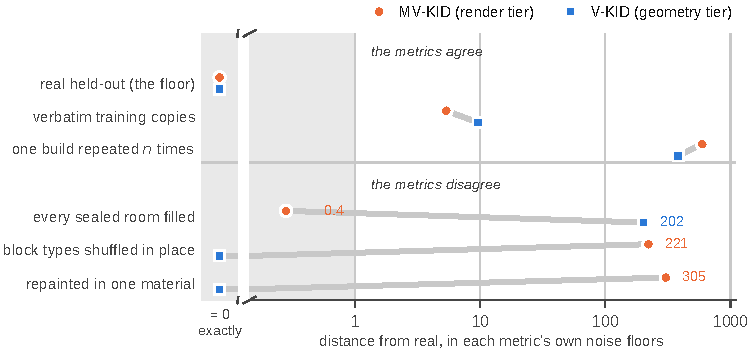
\includegraphics[width=0.88\linewidth]{figures/fig10_ladder}
\caption{\textbf{Two metrics, one run, eight rungs of known damage.} Each rung's distance
from held-out real, in that metric's own noise floors ($n{=}128$, symlog). The geometric metric's two material rungs are bit-identical to real, not merely small,
so they sit in a separate gutter. The band marks one noise floor; per-statistic numbers are in
Table~\ref{tab:seven}.}
\label{fig:ladder}
\end{figure}

\subsection{It Is the View Protocol, Not the Encoder}
\label{sec:ablation}

\begin{figure}[t]
\centering
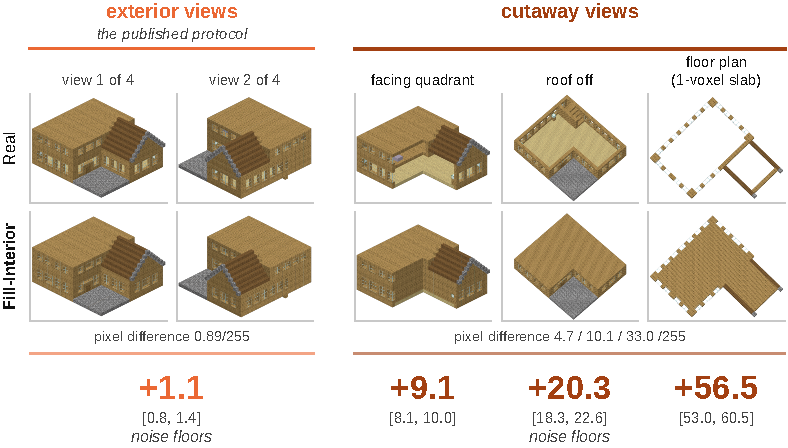
\includegraphics[width=0.90\linewidth]{figures/fig9_cutaway}
\caption{\textbf{The same encoder and statistic, only the views changed.} Each pair is a
held-out build over its \solidify{} twin. \emph{Left:} two of the four exterior views the
standard protocol renders, indistinguishable for this build at a mean pixel difference of $0.89/255$. \emph{Right:} three cutaway protocols on the same builds, each with its separation in
noise floors. DINOv2-B,
unbiased KID, $n{=}256$ against $512$ reference builds; full ablation in
Table~\ref{tab:ablation}.}
\label{fig:cutaway}
\end{figure}

%TL;DR of paragraph: varying encoder, view budget, projection and pooling changes nothing.
The finding could indict DINOv2 at four views rather than render-and-embed as a class. It
does not (Figure~\ref{fig:cutaway}, Table~\ref{tab:ablation}). Four other encoders land in the same $0.04$--$0.18$ band as our DINOv2-B: CLIP ViT-B/16 and B/32, ImageNet-supervised ResNet-50,
and the Inception network FID itself uses. Quadrupling the cameras does not help either.
\textbf{Sixteen views covering roof and underside separate the probe \emph{less} well
than four} ($+0.08$ against $+0.18$), which is what added views carrying no information about the
quantity should do. Perspective projection reads $+0.06$. Nothing measured on exterior views reaches a
quarter of one noise floor.

%TL;DR of paragraph: the cutaway rows are the positive control that makes this a statement about information rather than features.
The cutaway rows are the positive control. The same encoder and the same statistic recover
the interior at up to fifty times the separation once the view protocol stops hiding it,
which makes this a statement about \emph{information} rather than about features:
\textbf{the standard view protocol does not put interior structure into the image, so no
encoder downstream of it can score that structure.} A cutaway is not itself a good metric,
because a section view discards the facade the render tier exists to read.

\subsection{Both Directions, a Second Domain, and a Theorem}
\label{sec:hollow}

%TL;DR of paragraph: hollowing is as invisible as filling, so the blindness runs along the whole interior axis, and separations compare within a run.
The corruption this field actually produces is the converse of \solidify{}: the hollow
shells that surface-fitted mesh and implicit generators emit. It is equally invisible. In
the converse-probe run at $n{=}128$, \mvkid{} places \hollow{} at $+0.4$ noise floors and
\solidify{} at $+1.0$ against a real-vs-real floor of $+0.0$, while \vkid{} places the same
two arms at $+156.0$ and $+286.7$. The render metric is blind along the whole interior axis
rather than to one hand-built probe. Under our translucent renderer neither direction
separates at the protocol's $n{=}128$. Each run estimates its own noise floor, which is why \solidify{}
reads $286.7$ here and $201.80$ in the leaderboard run: separations compare within a run
(Appendix~\ref{app:nscale}).

%TL;DR of paragraph: the LEGO replication reproduces the qualitative structure, with the appearance controls firing on the same builds.
\label{sec:lego}The pattern is not a property of Minecraft houses. On the LEGO corpus at
$n{=}256$, with the domain pictured in Figure~\ref{fig:lego}, \mvkid{} places the solidified arm at $\mathbf{-0.01}$
noise floors, \emph{below} the real floor, while \vkid{} places it at $\mathbf{+118.6}$. On
the same builds at the same $n$ the render metric separates \matshuffle{} at
$\mathbf{+140.0}$ floors and \monochrome{} at $\mathbf{+685.8}$, so it resolves appearance
damage on this corpus and still cannot see the interior.

%TL;DR of paragraph: under an opaque renderer the invisibility is exact, which makes it a theorem rather than a measurement.
Whether interior damage reaches the image at all depends on the renderer. Under an
\emph{opaque} renderer it provably does not: filling sealed air cannot alter any exterior
view, so no encoder and no statistic can separate it at any sample size. Rendered opaquely,
all $1{,}024$ held-out (build, view) pairs we test are bit-identical, and
Appendix~\ref{app:hull} gives the proof.

%TL;DR of paragraph: our renderer leaks through translucency rather than doorways, and every changed pixel sits inside a bit-identical silhouette.
Our default renderer is not opaque, and under it \solidify{} alters $\mathbf{91\%}$ of the
$1{,}596$ test-split views, touching a median $1.2\%$ of pixels at a median maximum channel difference of $103/255$. What leaks is \emph{translucency}, not doorways:
air reachable through a doorway is never sealed, whereas a glass block in front of a filled
void does show the fill. Every changed pixel lies inside the silhouette, and the silhouette
is bit-identical (Appendix~\ref{app:hull}).

\subsection{Complementary Blindness Forces the Aggregation Rule}
\label{sec:complementary}

\begin{table}[t]
\centering
\small
\setlength{\tabcolsep}{3pt}
\caption{\textbf{The leaderboard.} Appearance and geometry are in noise floors of that pillar's own in-run real-vs-real spread, and
\blockscore{} is the \textbf{maximum} across five pillars. The three pillars that never
determine the maximum here use a coarser in-run scale and are reported in
Appendix~\ref{app:tables}. $\dagger$~marks the contaminated checkpoint of \S\ref{sec:casestudy}, unrankable and shown for comparison.}
\label{tab:leaderboard}
\begin{tabular}{rlrlrr}
\toprule
& arm & \blockscore{}~$\downarrow$ & worst pillar & appearance & geometry \\
\midrule
  & \realheld{} \emph{(anchor)}      & $0.00$   & ---        & $+0.00$   & $+0.00$ \\
\midrule
\multicolumn{6}{l}{\emph{submissions}} \\
$\dagger$ & \voxar{} \emph{(contaminated)} & $106.87$ & geometry & $+69.76$ & $+106.87$
\\
1 & \voxar{} \emph{(clean)} & $\mathbf{136.73}$ & geometry & $+85.31$ & $+136.73$ \\
2 & \llmft{} & $149.19$ & appearance & $+149.19$ & $+137.72$ \\
3 & \llmgeo{} & $191.88$ & appearance & $+191.88$ & $+145.58$ \\
4 & \patchstitch{} & $246.15$ & appearance & $+246.15$ & $+183.03$ \\
5 & \gabled{} & $300.15$ & geometry & $+287.97$ & $+300.15$ \\
6 & \hollowbox{} & $476.22$ & appearance & $+476.22$ & $+312.39$ \\
7 & \randomvox{} & $603.09$ & appearance & $+603.09$ & $+344.94$ \\
\midrule
\multicolumn{6}{l}{\emph{probes and controls: known damage, not submissions}} \\
  & \textbf{\solidify{}} & $201.80$ & geometry & $\mathbf{+0.14}$ & $\mathbf{+201.80}$ \\
  & \matshuffle{} & $231.52$ & appearance & $+231.52$ & $\mathbf{+0.00}$ \\
  & \monochrome{} & $297.95$ & appearance & $+297.95$ & $+0.00$ \\
  & \copynoise{} & $302.73$ & geometry & $+153.53$ & $+302.73$ \\
\midrule
\multicolumn{6}{l}{\emph{disqualified: refused a rank, with the reason}} \\
  & \singlemode{}                    & DQ & \multicolumn{3}{l}{mode collapse, $+45.1$ spreads on voxel diversity} \\
  & \traincopy{}                     & DQ & \multicolumn{3}{l}{memorization, $+10.7$ spreads on retrieval percentile} \\
  & \voxarun{} \emph{(clean)}        & DQ & \multicolumn{3}{l}{memorization, $+3.0$ spreads, at duplicate rate exactly $0.000$} \\
\bottomrule
\end{tabular}
\end{table}

%TL;DR of paragraph: each tier is fooled by the corruption aimed at it and rescued by the other, and the asymmetry between the two failures is large.
Table~\ref{tab:leaderboard} shows the complementarity directly. \solidify{} reads $+0.14$ on appearance against $+201.80$ on geometry, a factor of
$1{,}441$ between two pillars scoring the same arm, and \matshuffle{} is the converse,
$+231.52$ on appearance against \emph{exactly} $+0.00$ on geometry. Each tier is fooled by the corruption aimed at it and
rescued by the other, which is why \blockscore{} takes the worst pillar. The two failures
differ in severity: the best attack we have on \vkid{} is \patchstitch{}, which buys
near-perfect local occupancy statistics with globally incoherent structure and improves its geometry pillar over its appearance pillar by only $1.3\times$ ($+183.03$
against $+246.15$).

%TL;DR of paragraph: the geometric separation does not come from the added mass or from the sealed-interior scalar.
\vkid{} does not separate \solidify{} through the added mass, nor through the
sealed-interior scalar the probe drives to zero. Deleting the explicit size term moves the
separation from $201.8$ to $202.2$ floors, deleting the sealed-interior scalar moves it to
$197.1$, and deleting both leaves $197.3$. No single block of the descriptor reproduces the
result alone, the best being the scalar panel at $164.5$ (Appendix~\ref{app:descriptor}).

%TL;DR of paragraph: a mass-matched control separates on the render metric and not the geometric one, which is the dissociation stated without a probe-specific argument.
The sharper test is a control matched on the quantity in question. \growshell{} dilates the
solid outward until it has added \emph{exactly} the number of blocks \solidify{} adds to
that build, which it achieves to within one block on $128$ of $128$ builds at a median of
$196$. Same builds, same material, same mass, and the only difference is whether the new
mass goes inside or outside. The two metrics then part company completely. In that run
\mvkid{} places \growshell{} at $\mathbf{+102.3}$ noise floors and \solidify{} at
$\mathbf{+0.3}$, while \vkid{} places them at $214.5$ and $201.8$. A metric that counted
blocks could not produce that pair of rows, because the block count is the one thing the
two arms share.

%TL;DR of paragraph: the two tiers disagree about real uncorrupted builds too, and how a squared statistic is read is a separate correction.
The two tiers disagree about real, uncorrupted builds as well, with no probe involved: ranking the same $128$ held-out builds
by each metric's exact per-build contribution gives two nearly independent orderings, and
only the geometric one tracks how much interior a build has (Figure~\ref{fig:influence}).
Separately, because these statistics are squared, an arm that fails on a quarter of its
builds scores only $6.4\%$ of the way to fully bad; reporting the square root recovers the failure rate to a mean absolute error of $0.013$
against $0.128$
(Appendix~\ref{app:failrate}).

\subsection{Case Study: Contamination No Statistic Sees}
\label{sec:casestudy}

%TL;DR of paragraph: the case study asks whether the suite catches a failure we did not build, and a required provenance declaration finds it in three arms where every distribution statistic reads clean.
The results above use corruptions we built, where ground truth is known by construction.
This case study asks whether the suite catches a failure we did not build. A generator we
control is the right subject, because its training split is knowable. The suite requires
every arm to declare that split. \voxar{}, the top-ranked submission, declared one that
contained $346$ of the $399$ canonical test builds
($87\%$). \label{sec:casestudy:llm}\llmft{} and \llmgeo{} declared an earlier $90/10$
shuffle holding $53$ of the $399$ ($13\%$). No distribution statistic sees either.
\voxar{}'s duplicate rate is $0.000$ and its retrieval percentile $0.496$ against a real
held-out floor of $0.540$, far from the verbatim-copy control at $+10.7$ spreads.

%TL;DR of paragraph: retraining on the clean split erases the margin and turns the cross-track result into a tie, and the gate disqualifies the sibling checkpoint.
Retraining \voxar{} on the canonical split, with architecture and hyperparameters
unchanged, isolates the effect (Figure~\ref{fig:contamination}). We report raw \vkid{} here,
because the contaminated and clean runs do not share a noise floor. Contaminated, the arm
scores $11.62$ and separates from one language-model baseline at Holm
$5.5{\times}10^{-3}$; clean, it scores $14.898$ against their $15.006$ and $15.869$ and
separates from neither. Under a correctly calibrated test it never held a significance group
alone (Appendix~\ref{app:significance}). Contamination lowers an arm's distance from real,
so the baselines' own contamination flatters them and we report that comparison as not
separated. The gate also caught the sibling: \voxarun{}, retrained on the same clean split,
is disqualified at $+3.0$ spreads on a retrieval percentile of $0.369$ against a real floor
of $0.540$, at a duplicate rate of exactly $0.000$.

%TL;DR of paragraph: a required field beats every detector, and the two tracks fail on different pillars, which is the maximum rule acting on real submissions.
The result bears on the paper's argument twice. What detected both contaminations was a
required field rather than a detector: every memorization gate passed and the declaration
did not, so benchmarks in this domain should require that declaration and refuse to rank
arms that cannot make it. The second bearing is on aggregation. The clean \voxar{} is
geometry-limited, $+136.73$ geometry against $+79.90$ appearance, and both language-model
arms are appearance-limited, so a mean over pillars would have reported them as one model
at two quality levels (Appendix~\ref{app:tables}).

\subsection{Human Evaluation}
\label{sec:human}

%TL;DR of paragraph: the study, its three pre-registered pairs, and the exclusion rule.
Synthetic corruption shows only that the metrics order damage we built ourselves. Human
judgment is the other check. Twenty raters, naive to the hypothesis, each compared $48$ label-stripped
pairs rendered exactly as the metric renders them, yielding $912$ judgements after one
session was excluded on catch trials. Three predictions were recorded in the instrument
before any rater saw a page (Appendix~\ref{app:study}).

%TL;DR of paragraph: raters are at chance on the exterior pair and above chance on the cutaway, so the blindness is informational rather than a defect of the metric.
\textbf{The corruption is invisible to people too.} On exterior views raters preferred the
real build over its solidified copy on $43$ of $84$ trials, $0.512$ $[0.407, 0.616]$:
chance. This decides what kind of failure this is. Had people separated what the metric
could not, the metric would be failing to read something a reader reads. They cannot, so
the information is absent from the picture rather than discarded by the statistic.
\textbf{The same people separate the same builds once the view exposes the interior}, $69$
of $90$, $0.767$ $[0.669, 0.842]$, which turns ``nobody can tell'' into ``nobody can tell
\emph{from this view}''. The converse probe is also at chance, $0.606$ $[0.437, 0.753]$ on
$33$ trials.

%TL;DR of paragraph: the pre-registered pair reverses unanimously, and the geometric scalars say why.
\textbf{The pre-registered pair reversed, unanimously.} Both metrics rank \patchstitch{}
above \gabled{}; raters chose \gabled{} on \textbf{$93$ of $93$} trials $[0.960, 1.000]$.
The geometric scalars say why, and neither side is making an error. \gabled{} is a genuine
statistical outlier, a hollow and almost perfectly symmetric shell at $0.562$ open interior
ratio against a real $0.129$, so the metrics are right that it is far from the real
distribution. \patchstitch{} is assembled from patches of real builds, so its local
statistics are real by construction and only its global structure is wrong, which its
largest-connected-part ratio of $0.866$ records against a real $0.978$
(Table~\ref{tab:baselines}). A distribution distance over local features therefore rewards
\emph{statistically} house-like over \emph{recognizably} a house.

\subsection{Limitations}
\label{sec:limitations}

%TL;DR of paragraph: one renderer is the sharpest remaining gap, and the geometric tier is attackable and material-blind.
We measure two corpora and \emph{one renderer}. The renderer is the sharper gap, and the
invisibility is a
theorem about opaque rendering rather than a fact about our rasterizer
(Appendix~\ref{app:hull}), and what would close the gap is to push identical builds and the
identical probe through a path tracer sharing no code with ours. \vkid{} is a
local-statistics descriptor, and \patchstitch{}, built to exploit that, \emph{outranks} the
coherent but simple \gabled{} on both tiers, an ordering raters reverse unanimously
(\S\ref{sec:human}). That is the clearest limitation of the geometric tier, so
\patchstitch{} stays a standing control. \vkid{} is also blind to materials by
construction, which is why the suite has two tiers and neither number belongs alone.

%TL;DR of paragraph: the leaderboard runs at half the protocol's own n, and we score no published external model.
\textbf{Our own protocol asks for $n \geq 256$ and the leaderboard runs at $n{=}128$},
because the generator arms were sampled at $128$; the encoder and view ablation and the
LEGO replication are at $n{=}256$. We also score no published external model, so the
leaderboard demonstrates what the suite does rather than re-ranking a published result. The
one external comparison available without retraining is to a protocol rather than to a
model: the generator released with this corpus \citep{chen2019voxelcnn} reports a
cumulative chamfer distance, which is exactly invariant to our probe
(\S\ref{sec:related}).
